%
% xstern.tex
%
% (c) 2024 Prof Dr Andreas Müller
%
\begin{figure}
\centering
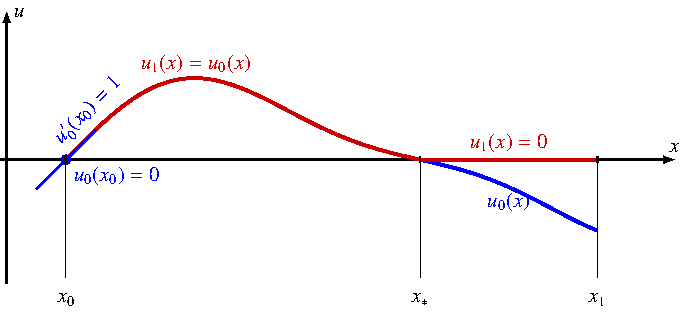
\includegraphics{chapters/060-variation2/images/xstern.pdf}
\caption{Konstruktion der Funktion $u_1(x)$ für das Jacobi-Kriterium.
Die Funktion $u_0(x)$ ist Lösung der Jacobi-Differentialgleichung
\eqref{buch:variation2:jacobi:eqn:jacobisl}.
Die Funktion $u_1(x)$ stimmt bis zur Nullstelle $x_*$ von $u_0(x)$ mit
$u_0(x)$ überein, für $x>x_*$ verschwindet sie.
\label{buch:variation2:fig:xstern}}
\end{figure}
